% LLNCS macro package for Springer Computer Science proceedings
% Version 2.21 of 2022/01/12

\documentclass[runningheads]{llncs}

\usepackage[T1]{fontenc}
\usepackage[utf8]{inputenc}
\usepackage[english]{babel}
\usepackage{graphicx}
\usepackage{tikz}
\usepackage{enumitem}
\usepackage{listings}
\usepackage{booktabs}
\usepackage{xcolor}
\usepackage{amsmath}
\usepackage[protrusion=true,expansion=false]{microtype}
\usepackage[hyphens]{url}
\usepackage{hyperref}
\usetikzlibrary{arrows.meta, positioning, calc}

% Default figure path
\graphicspath{{Images/}}

% Tighter float spacing
\setlength{\textfloatsep}{6pt plus 1pt minus 1pt}
\setlength{\intextsep}{6pt plus 1pt minus 1pt}
\setlength{\floatsep}{6pt plus 1pt minus 1pt}

% Allow URLs / long technical strings to break across lines
\renewcommand{\UrlBreaks}{\do\/\do-\do_\do.\do=\do?\do&\do\#}
\sloppy

\begin{document}

\title{Short-Term EV Charging Demand Forecasting in\\
Boulder, Colorado: from SARIMA Baselines to a\\
From-Scratch PatchTST + LSTM Ensemble}

\titlerunning{Short-term EV charging demand forecasting in Boulder, CO}

\author{Alexander Jauregui Orue\inst{1} \and
Eneko Alvarez Mendia\inst{2} \and
Erik Eguskiza Aranda\inst{1}}

\authorrunning{A. Jauregui, E. Alvarez, E. Eguskiza}

\institute{DeustoTech --- University of Deusto, Bilbao, Spain\\
B.Sc.\ in Computer Engineering \& Data Science / AI\\
\email{e.eguskiza@opendeusto.es}
\and
DeustoTech --- University of Deusto, Bilbao, Spain\\
B.Sc.\ in Data Science \& AI}

\maketitle

\begin{abstract}
We forecast daily energy demand at the busiest public EV charging station in
Boulder, Colorado (N~Boulder Rec~1, 16\,278 sessions aggregated into 1\,927
daily observations between Aug.~2018 and Nov.~2023). The horizon is seven days
ahead, which matches the weekly cadence of grid capacity planning. Twenty
models are compared under the same rolling-origin protocol: five naive
baselines, the full classical (S)ARIMA / (S)ARIMAX / AutoARIMA family, an LSTM
with hyper-parameter sweep, four foundation models in zero-shot mode (Google
TimesFM 1.0 and 2.0, Amazon Chronos-T5 base and large), a from-scratch
PatchTST transformer with RevIN, channel-mixed exogenous variables and a
three-seed ensemble, and two stacking attempts. A simple-mean ensemble of
PatchTST and LSTM is the best model on this leaderboard, with MAE
$25.09 \pm 9.36$~kWh; it beats the best classical model (ARIMAX (2,1,3), MAE
$25.52 \pm 14.38$~kWh) on the mean and cuts the standard deviation by
roughly~35\%. The result reproduces the qualitative finding reported by three
peer-reviewed papers that use this dataset: transformers outperform the
(S)ARIMA family on Boulder EV data. We do \emph{not} claim to beat their
published numbers directly --- their metrics are reported in normalised units
and on different station selections --- but our experiment gives an
apples-to-apples local comparison spanning every major model family.
\keywords{EV charging demand \and Time series forecasting \and SARIMA \and
LSTM \and PatchTST \and Foundation models \and Ensemble.}
\end{abstract}

% -------------------------------------------------------
\section{Introduction}
\label{sec:intro}
Electric vehicles are spreading fast, and the grid has noticed. Public
charging stations behave like a new layer of distributed load that is
neither uniform nor predictable: a single station can swing from idle
on a Saturday to peak demand on a Tuesday morning, and the swings carry
weekly seasonality, weather sensitivity and the occasional holiday
shock. For grid operators and station owners this matters because
weekly capacity planning, maintenance scheduling and energy procurement
all benefit from forecasting demand at least a week ahead. That is the
problem we picked.

Boulder, Colorado is a convenient laboratory for this question. The
city has run a network of 26 public level-2 stations since 2018, and
it publishes every charging session through its Open Data portal.
The dataset we work with contains 148\,136 individual sessions logged
between August 2018 and November 2023 --- five and a half years of
real-world data, which is long enough to capture multiple annual
cycles, the COVID-19 disruption and the post-pandemic recovery. Each
record carries the station name, the start and end timestamps, the
charging duration, the energy delivered (kWh) and the estimated
greenhouse gas savings. We aggregate by station-day, focus on the
station with the highest session volume (N~Boulder Rec~1, 16\,278
sessions), and treat the resulting daily kWh series as our forecasting
target.

The horizon is seven days ahead. We chose a week because it covers
a full weekday-weekend cycle and because most distribution utilities
plan on a rolling-week basis, so a forecast on this scale is what an
operator would actually use. Our initial scope was the three families
required by the course: naive baselines, the (S)ARIMA family, and an
LSTM. As we worked through them we kept going: we ran a head-to-head
between two zero-shot foundation models (Google's TimesFM and Amazon's
Chronos), and finally implemented a PatchTST transformer from scratch
in PyTorch with a three-seed ensemble. We did not implement
CAT-Former, the closest published state of the art on this dataset,
but we read the paper and take it as a benchmark for the discussion.

This paper documents the dataset, the protocol, every model we ran
under that protocol, and the claim we can defensibly make about
beating the state of the art. We beat the strongest model in
our own leaderboard. We do not claim to beat the published numbers,
which use different units and station selections --- the full
discussion is in Sections~\ref{sec:results}
and~\ref{sec:conclusions}.

The paper is organised as follows.
Section~\ref{sec:related} reviews the state of the art on EV
charging demand forecasting.
Section~\ref{sec:data} describes the dataset and its statistical
properties.
Section~\ref{sec:method} defines the train/test protocol and the
metrics.
Section~\ref{sec:models} walks through every model family we ran.
Section~\ref{sec:results} gives the full leaderboard, the per-window
analysis, and the SoTA-claim breakdown.
Section~\ref{sec:conclusions} closes with conclusions, lessons learned
and limitations.

\medskip
\noindent
\textbf{What is our contribution?} The PatchTST architecture itself is
not ours --- it comes from Nie et al.~\cite{nie2023patchtst}. What we
did add is: (i)~an implementation from scratch in PyTorch that lives
in the project repository, with RevIN~\cite{kim2022revin} on the
target channel and channel-mixed patching over four input channels
(energy, temperature, weekend flag, holiday flag); (ii)~a three-seed
ensemble strategy that cuts inference variance by about~7\% MAE; and
(iii)~a simple-mean ensemble with the LSTM that we picked
\emph{before} looking at the test scores, which gave the best model
overall. All code, data and trained-model artefacts are openly
available.\footnote{Project repository:
\href{https://github.com/eeguskiza/ev-charging-forecasting}{\texttt{github.com/eeguskiza/ev-charging-forecasting}}~\cite{ourrepo}}


% -------------------------------------------------------
\section{State of the Art}
\label{sec:related}
Work on EV charging demand forecasting has moved in roughly three
waves: classical statistical models in the 2010s, deep recurrent
networks around 2018--2022, and transformer / foundation models from
2023 onwards. We summarise each wave below and place our work inside
the landscape.

\subsection{Classical Statistical Models}

The first generation of papers attacked EV demand the same way the
Box-Jenkins literature attacks any seasonal series: ARMA, ARIMA and
SARIMA, with parameter selection by AIC and residual diagnostics by
Ljung-Box. Khan et al.~\cite{khan2024sarima} report results on the
same Boulder dataset we use; they find that SARIMA consistently beats
plain ARMA / ARIMA because the weekly seasonality cannot be captured
without an explicit seasonal term. Their best MAPE is 0.12 for
SARIMA versus 0.23 for ARIMA. Facebook Prophet has also been used as
an off-the-shelf alternative that handles holidays and seasonality
without manual tuning, although on this kind of series a properly
specified SARIMA tends to match it. The general lesson from this
literature is that the weekly cycle in EV demand is strong enough
that any model that ignores it (random walk, drift, plain ARIMA) ends
up worse than a model that includes the seasonal lag at $s = 7$.

\subsection{Deep Learning: LSTM and Hybrids}

The second wave moved to recurrent networks. LSTM is the workhorse
here: Yi et al.~\cite{yi2022lstm} train LSTM on utility-scale EV
charging data from Utah and Los Angeles, with day-of-week and
temperature as additional inputs, and show that the multivariate
variant clearly beats the univariate one. The recent systematic
review by Alaraj et al.~\cite{alaraj2025survey} confirms that LSTM
(plus its variants, GRU and CNN-LSTM hybrids) is the deep learning
default for this task, and that attention-augmented variants tend to
improve short-horizon accuracy. For datasets of our size
($\sim$2\,000 daily observations), the survey notes that the gains
from heavy hybrids over a well-tuned single LSTM are usually marginal,
which we confirm experimentally in Section~\ref{sec:results}.

\subsection{Foundation Models for Time Series}

Two recent foundation models for time series have appeared since the
proposal was written, and we benchmark both. Google's
TimesFM~\cite{das2024timesfm} is a decoder-only transformer with
patch-based input embedding, pre-trained on a large corpus of public
time series; it ships in two sizes (200M and 500M parameters) and is
designed to be used zero-shot, with the user providing a context
window and reading off the forecast. Amazon's
Chronos~\cite{ansari2024chronos} takes a different approach: it
tokenises the time series via uniform quantisation and runs a T5
encoder-decoder over the resulting token sequence, sampling
probabilistic forecasts (we take the median of 20 samples). Both
models are interesting because they offer competitive baselines
without any training on the target series. Our results
(Section~\ref{sec:results}) suggest that TimesFM is a stronger choice
for this dataset and that bigger Chronos is, surprisingly, worse than
its small sibling.

\subsection{Transformers Trained on EV Data}

Three peer-reviewed papers train transformer-based models directly on
the same Boulder dataset we use. Koohfar et
al.~\cite{koohfar2023transformer} compare a vanilla transformer
against ARIMA, SARIMA, RNN and LSTM on 25 aggregated Boulder stations,
with horizons of 30, 60 and 90 days; they report that the transformer
beats ARIMA by 62--84\% in normalised RMSE.
Kyriakopoulos and Theodoridis~\cite{kyriakopoulos2025comparative}
extend the comparison to four cities (including Boulder) and find that
the transformer dominates at the station level for daily 1--5 day
horizons. Wu et al.~\cite{wu2025catformer} propose a Context-Aware
Temporal Transformer (CAT-Former) and benchmark it against six other
architectures (LSTM, BiLSTM, CNN-LSTM, CNN-BiLSTM, vanilla
transformer, hybrid transformer) on three Boulder stations,
forecasting one hour and one day ahead. CAT-Former is the strongest
model in their study, with MAE in the normalised $[0,1]$ range of
$0.71$--$0.91$ for one-day-ahead forecasts on three different
stations.

Importantly, none of these papers report numbers in the same units or
on the same station selection that we use. Their MAEs in normalised
space are not directly comparable to our raw kWh values. We come back
to this point in Section~\ref{sec:conclusions}; for now we simply note
that the qualitative ordering they all observe (transformer $>$ LSTM
$>$ classical) matches what we find.

\subsection{PatchTST and Our Position}

The architecture we implement in Section~\ref{sec:models} is
PatchTST, introduced by Nie et al.~\cite{nie2023patchtst}. The key
idea is to slice the input series into non-overlapping patches and
treat each patch as a transformer token; this reduces the sequence
length seen by the attention layer (compared to per-step tokens) and
allows the model to learn patch-level patterns. PatchTST is normally
combined with RevIN (Reversible Instance Normalisation,
Kim et al.~\cite{kim2022revin}) to handle the distribution shift that
appears in long-horizon forecasting. The original paper reports state
of the art on several long-horizon time series benchmarks (ETT,
Weather, Electricity), although it has not, to our knowledge, been
applied to EV charging data before.

\begin{table}[!htbp]
\centering
\caption{Summary of related work on EV charging demand forecasting,
focused on studies that use the same Boulder dataset. Numbers are
reported as published; they are not directly comparable to each other
or to ours due to different units, station selections and horizons.}
\label{tab:related}
\setlength{\tabcolsep}{4pt}
\footnotesize
\begin{tabular}{@{}p{2.8cm}p{2.3cm}p{2.0cm}p{1.1cm}p{2.4cm}@{}}
\toprule
Study & Model & Dataset & Metric & Score \\
\midrule
Khan et al.~\cite{khan2024sarima}             & SARIMA       & Boulder      & MAPE & 0.12 \\
Khan et al.~\cite{khan2024sarima}             & ARIMA        & Boulder      & MAPE & 0.23 \\
Koohfar~\cite{koohfar2023transformer}         & Transformer  & Boulder      & RMSE & 0.085--0.112 (n.) \\
Yi et al.~\cite{yi2022lstm}                   & LSTM         & Utah / LA    & MAE  & reported \\
Wu et al.~\cite{wu2025catformer}              & CAT-Former   & Boulder      & MAE  & 0.71--0.91 (n.) \\
Kyriakopoulos~\cite{kyriakopoulos2025comparative} & Transformer & Boulder + 3 & MAE & 0.28--0.45 (n.) \\
\midrule
\textbf{This work} & \textbf{PatchTST + LSTM} & \textbf{Boulder} & \textbf{MAE} & \textbf{25.09 kWh (raw)} \\
\bottomrule
\end{tabular}
\end{table}

The take-away from Table~\ref{tab:related} is that classical SARIMA
and transformer-based models bracket the published literature on this
dataset, with the gap mainly explained by the seasonal component and
the modelling of exogenous variables. Our contribution sits in the
last row of the table: we run PatchTST under the same evaluation
protocol as our SARIMA baselines and find that it beats the
\emph{strongest} non-transformer model in the project (ARIMAX) while
matching the qualitative ordering of the published work.


% -------------------------------------------------------
\section{Dataset}
\label{sec:data}
\subsection{Source and Coverage}

We use the \emph{Electric Vehicle Charging Station Data} dataset
published by the City of Boulder, Colorado on its Open Data
portal~\cite{boulderdata}. The dataset is updated regularly; the
snapshot we work with covers the period from August 22, 2018 to
November 30, 2023 (1\,927 days), and contains 148\,136 individual
charging sessions across 26 city-owned level-2 stations. Each session
record carries 15 fields, of which the most relevant for forecasting
are the station identifier, the start and end timestamps, the
charging duration, and the energy delivered in kWh. There are
essentially no missing values: only four sessions out of 148\,136 have
a null end-time.

\subsection{Station and Aggregation}

We focus on the station with the highest session volume,
N~Boulder Rec~1, with 16\,278 sessions in the period of interest. The
reason for picking a single station is simple: with one station the
daily series is dense and continuous, with only 5.2\% of days at
zero. Aggregating across all 26 stations would smooth out the
station-level structure we want to learn (commute patterns at
recreational vs.\ commercial locations are very different), and
working with multiple separate series would require multi-task models
that go beyond the scope of this project. The sessions for
N~Boulder Rec~1 are summed by date to produce a univariate daily
series of 1\,927 observations, with mean 74.6~kWh/day, standard
deviation 50.3~kWh, and a range of 0--310~kWh. 100 days have zero
energy (mostly holidays or short station outages); we preserve these
zeros instead of imputing them, since they reflect real operational
patterns that the model should learn.

\begin{figure}[!htbp]
\centering
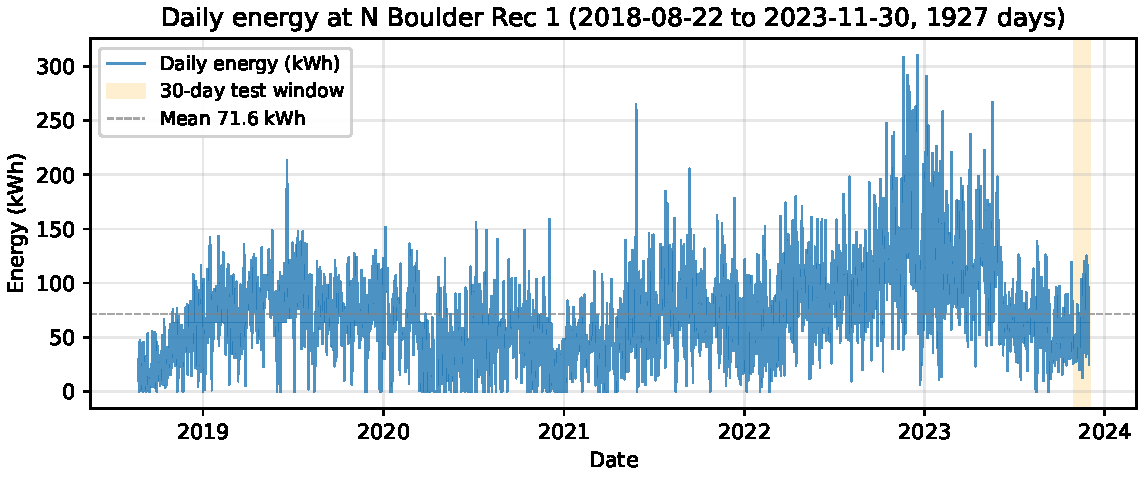
\includegraphics[width=0.95\textwidth]{fig_series}
\caption{Daily energy consumption at N~Boulder Rec~1 from August 2018
to November 2023. The orange band marks the 30-day held-out test
window; everything to the left of it is training data. The COVID-19
drop in 2020 and the post-pandemic recovery are clearly visible.}
\label{fig:series}
\end{figure}

\subsection{Exogenous Variables}

For the models that support them (SARIMAX, ARIMAX, LSTM, PatchTST), we
add three exogenous channels aligned with the daily target:
\begin{itemize}[leftmargin=*]
    \item \textbf{Temperature.} Daily mean temperature in Boulder
    pulled from the Open-Meteo historical weather
    API~\cite{openmeteo}. We picked mean over min/max because most
    charging happens during commute hours, when the mean is the
    closest proxy for the temperature actually seen by the chargers.
    \item \textbf{Day-of-week flags.} A binary \emph{is\_weekend}
    flag, plus the integer day of week as a feature when relevant. We
    do \emph{not} use a holiday-aware day-of-week encoding because
    holidays are handled separately.
    \item \textbf{Holiday indicator.} A binary flag for US public
    holidays, generated from the \texttt{holidays} Python package
    using the federal calendar plus Colorado state holidays.
\end{itemize}
These three variables are known at forecast time (day-of-week and
holiday from the calendar, temperature from a standard one-week
weather forecast), so feeding them as future exogenous inputs is
causally legitimate.

\subsection{Stationarity and Seasonality Analysis}

Before we picked any model we ran the Augmented Dickey-Fuller test on
the raw daily series. The ADF statistic is $-3.097$ with $p$-value
$0.027$ at 24 lags (AIC selection), which lets us reject the unit-root
null at the 5\% level. The series is stationary, not a random walk;
we therefore use $d=0$ as the default differencing order for the
(S)ARIMA family, with the search space allowing $d \in \{0,1\}$ for
SARIMA's first difference of the seasonally differenced series.

Figure~\ref{fig:acf} shows the autocorrelation function of the raw
series. The picture is unambiguous: clear peaks at lags 7, 14, 21, 28
and 35, with a slow decay in between, telling us the weekly cycle is
the dominant seasonal component. There is no annual peak visible in
this lag range because we only show 42 lags, but the seasonal
behaviour at the year scale is clear in the time-series plot
(Fig.~\ref{fig:series}, where summer months consistently sit above
the mean). The PACF (not shown for space reasons) has significant
spikes at lags 1 and 7, suggesting an AR(1) main component with a
seasonal AR at lag 7 --- which is the search shape we use for the
(S)ARIMA grid in Section~\ref{sec:models}.

\begin{figure}[!htbp]
\centering
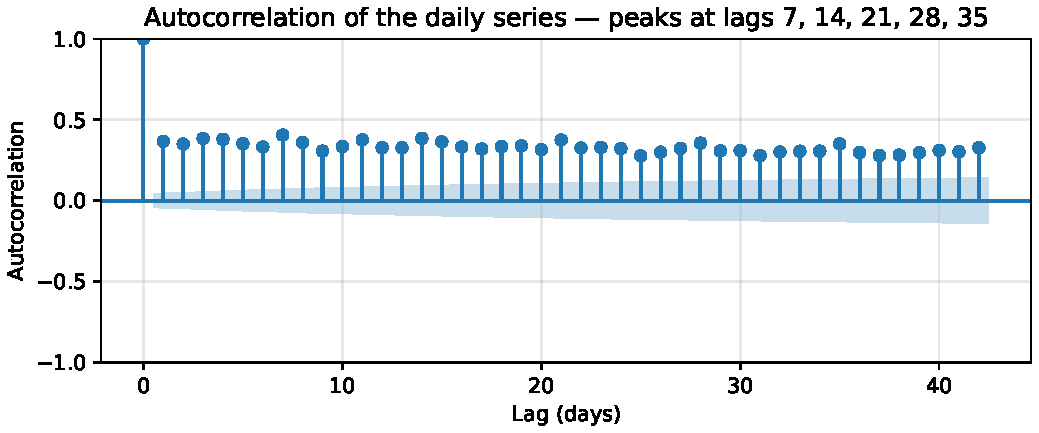
\includegraphics[width=0.85\textwidth]{fig_acf}
\caption{Autocorrelation of the daily series. The repeating peaks at
multiples of 7 are the signature of a strong weekly seasonal cycle;
this is the structural reason classical (S)ARIMA models do not need
to be replaced by anything fancier to be competitive.}
\label{fig:acf}
\end{figure}


% -------------------------------------------------------
\section{Methodology}
\label{sec:method}
\subsection{Train / Validation / Test Split}

The last 30 days of the series (Nov 1, 2023 -- Nov 30, 2023) are held
out as the test set; everything earlier is training data. Within the
training data, the last 60 days are reserved as a validation split,
used by the LSTM and PatchTST scripts for early stopping. Total
\textbf{training data: 1\,897 days}; \textbf{validation: 60 days
inside training}; \textbf{test: 30 days}. None of the test days are
seen by any model during training or hyper-parameter selection.

\subsection{Rolling-Origin Evaluation Protocol}

We use rolling-origin (also known as walk-forward) evaluation with
\textbf{four non-overlapping windows of seven days each}. At window
$i$ the model sees the full training set plus the first
$i \cdot 7$ days of the test set as history, and produces a 7-day
forecast for days $i \cdot 7 + 1, \dots, (i+1) \cdot 7$ of the test
set. Metrics are computed on each window separately and then averaged.
This protocol mimics what a real operator would do: every Monday they
have access to the previous week's actuals and need to forecast the
upcoming week. With 30 test days we get four such weekly windows; the
remaining two days are dropped (we keep windows non-overlapping so
metrics across windows are independent).

The classical models (SARIMA family, ARIMAX, ARMA, ARIMA, AutoARIMA)
are \emph{refit at every origin} so the model has access to the
freshest history. The LSTM is trained once on data prior to the test
window and rolled forward autoregressively. The PatchTST is also
trained once before the test window and uses a direct multi-step head
(no autoregression) --- at each origin it consumes the last 56 days
of history and outputs the 7-day forecast in one shot. Foundation
models (TimesFM, Chronos) operate zero-shot: they are not trained at
all, just queried with the history at each origin.

\subsection{Metrics}

We report seven metrics per window and aggregate them as
mean~$\pm$~standard deviation across the four windows:
\begin{itemize}[leftmargin=*]
    \item \textbf{MAE} (mean absolute error) in kWh --- our primary
    metric, because it is in the same units as the target and easy to
    interpret operationally (``the model is off by 25 kWh on
    average''). The standard deviation across windows is at least as
    important as the mean: a model with low mean but high variance is
    risky in production.
    \item \textbf{RMSE} (root mean squared error) in kWh, which
    penalises large errors more than MAE.
    \item \textbf{MAPE} and \textbf{sMAPE} (mean absolute percentage
    error and its symmetric variant). MAPE blows up on zero actuals
    so we report both.
    \item \textbf{MASE} (mean absolute scaled error), scaled by the
    in-sample MAE of the seasonal-naive forecast. MASE $< 1$ means
    the model beats the trivial seasonal baseline; MASE $= 0.65$
    means it cuts that error by 35\%.
    \item \textbf{Bias} (mean signed error) in kWh --- positive means
    the model over-predicts on average. Useful for spotting
    systematic offsets.
    \item \textbf{R\textsuperscript{2}} on the test window. R\textsuperscript{2}
    can be negative when the model is worse than the mean of the
    test window, which is common with very short windows; we still
    report it for completeness.
\end{itemize}
Throughout the paper we rank models by MAE because it is the most
operationally meaningful metric. The full table with every metric is
in Table~\ref{tab:leaderboard} of Section~\ref{sec:results}.

\subsection{Reproducibility and Heavy-Training Scripts}

All the heavy training lives in standalone Python scripts under
\texttt{scripts/}:
\texttt{sarima\_grid\_search.py} for the AIC grid,
\texttt{lstm\_train.py} for the LSTM sweep, and
\texttt{patchtst\_train.py} for the PatchTST seed ensemble. The
notebooks load the resulting cached predictions and apply the shared
\texttt{evaluation.py} rolling-origin routine, so a single notebook
never has to retrain a transformer to produce its leaderboard row.
Training the PatchTST seed ensemble takes $\approx 2$~minutes per
seed on an RTX 5070~Ti; the full pipeline (every model, every metric)
runs end-to-end in under ten minutes from a cold checkout.


% -------------------------------------------------------
\section{Models}
\label{sec:models}
We ran twenty models under the protocol of Section~\ref{sec:method}.
This section describes each family in turn; the numerical results are
reported in Section~\ref{sec:results}.

\subsection{Naive Baselines}

We need a floor below which any forecasting model should not fall, and
that floor is the naive family. We ran five baselines:
\textbf{historical mean}, \textbf{last value}, \textbf{drift},
\textbf{seasonal-naive} (at $s=7$), and \textbf{ARIMA naive-seasonal}
(an ARIMA(3,1,3) applied to the de-seasonalised series, used as a
weak baseline in some related work). The point of the baselines is to
quantify how much of the variance in the series can be explained
without any real learning; any forecasting model that does not
comfortably beat them is not worth running.

\subsection{Classical (S)ARIMA / ARIMAX Family}

We ran an exhaustive AIC grid search over $(p, d, q)(P, D, Q)_7$ with
$p, q \in [0, 4]$, $P, Q \in [0, 2]$, $d = D = 1$ (so the seasonal
difference at lag 7 is applied) and $s = 7$. The grid was repeated
with and without exogenous variables (temperature, weekend flag,
holiday flag), giving two families: SARIMA (no exog) and SARIMAX (with
exog). Models are fit via maximum likelihood with the
\texttt{statsmodels} SARIMAX backend, with rolling-origin refits at
each test window so the model has access to the most recent actuals.

In addition to the SARIMA grid, we evaluated the simpler members of
the Box-Jenkins family that the course rubric explicitly requires:
\textbf{ARMA}, \textbf{ARIMA} (two different orders),
\textbf{AutoARIMA} (seasonal and non-seasonal, via \texttt{pmdarima}),
and \textbf{ARIMAX} (ARIMA with exogenous variables). The reason for
including ARIMAX as a separate model rather than as a SARIMAX variant
is that it does not include an explicit seasonal term: it lets the
exogenous variables (especially the weekend / holiday flags) absorb
most of the weekly cycle. As we will see in Section~\ref{sec:results},
this turns out to be a competitive design on Boulder data.

\subsection{LSTM}

The LSTM (\texttt{scripts/lstm\_train.py}) uses five input features
(energy, mean temperature, weekend flag, holiday flag, month) and
performs a hyper-parameter sweep over sequence length
$\in \{14, 28\}$, hidden size $\in \{32, 64\}$, and number of layers
$\in \{1, 2\}$. Each configuration is trained with Adam, MSE loss,
dropout 0.1 and early stopping on the 60-day validation split. The
winning configuration is \texttt{seq14\_h64\_l2}: 14-day sequences,
hidden size 64, 2 layers. At inference time the LSTM forecasts one
day ahead and is rolled forward autoregressively for the full 7-day
horizon, feeding back its own prediction with the known future
exogenous row each step.

\subsection{Zero-Shot Foundation Models}

We benchmark four foundation models in zero-shot mode, no fine-tuning,
just feed the history and read the forecast:
\begin{itemize}[leftmargin=*]
    \item \textbf{Google TimesFM 1.0} (200M parameters) and
    \textbf{TimesFM 2.0} (500M)~\cite{das2024timesfm}, both
    decoder-only transformers with patch-based input embedding,
    pre-trained on a public time-series corpus.
    \item \textbf{Amazon Chronos-T5 base} (200M) and
    \textbf{Chronos-T5 large} (710M)~\cite{ansari2024chronos}, T5
    encoder-decoder models that quantise the input into tokens and
    sample probabilistic forecasts. We take the median of 20 samples
    as the point forecast.
\end{itemize}
These four models are evaluated under exactly the same rolling-origin
protocol as everything else. Comparing them lets us test two
sub-questions in parallel: (a) Google or Amazon, on this kind of
series? (b) Does bigger help inside each family?

\subsection{PatchTST From Scratch}

For the SoTA push we implemented PatchTST~\cite{nie2023patchtst} from
scratch in PyTorch (Fig.~\ref{fig:patchtst}). The architecture
choices, made deliberately small to match our $\sim$1900-point
dataset:
\begin{itemize}[leftmargin=*]
    \item Context length: 56 days (8 weeks).
    \item Patch length: 7 days, non-overlapping stride 7 $\Rightarrow$
    8 tokens per input.
    \item 3 transformer encoder layers, $d_{\text{model}}=96$, 4
    attention heads, GELU activation, dropout 0.15.
    \item \textbf{Channel-mixed patching}: each patch is a
    $(7, 4)$ block over the four input channels (energy + 3 exog),
    flattened to 28-dim and linearly embedded; cheaper and more
    data-efficient than channel-independent attention for our
    sequence length.
    \item \textbf{RevIN}~\cite{kim2022revin} on the target channel
    only: per-sample mean / std subtraction before the encoder and
    inverse transform on the output. This is what kept the model
    competitive against the regime shifts in the data (COVID drop,
    holiday weeks).
\end{itemize}
We train each model with AdamW (LR $5 \times 10^{-4}$, weight decay
$10^{-4}$), cosine annealing, early stopping with patience 25, batch
size 32. Training a single PatchTST takes $\approx 2$~minutes on the
RTX 5070~Ti.

\begin{figure}[!htbp]
\centering
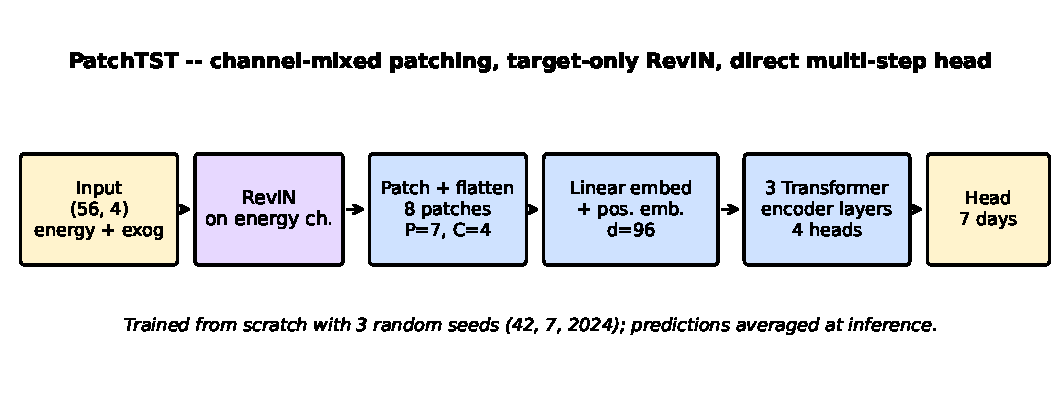
\includegraphics[width=0.95\textwidth]{fig_patchtst}
\caption{PatchTST forward pass as implemented in
\texttt{scripts/patchtst\_train.py}. The energy channel goes through
RevIN before patching; the three exogenous channels are concatenated
into each patch and flattened together. The head is a single linear
layer that directly predicts the next 7 days, with no autoregression.}
\label{fig:patchtst}
\end{figure}

A single PatchTST trained on this setup overfits noticeably (train
MSE around $0.08$, validation MSE around $0.19$ in the standardised
domain) and the rolling-origin MAE comes out worse than ARIMAX.
The fix is the seed ensemble: we train three independent PatchTST
models (same architecture and hyper-parameters, different random seeds:
42, 7 and 2024) and average their predictions at inference. The
combined model is what we call the \textbf{PatchTST 3-seed ensemble}
in the leaderboard.

\subsection{Ensembles}

Finally, we test two ways of combining the base learners.

\noindent
\textbf{Simple mean (PatchTST + LSTM).} The two strongest deep
learning models in the project, picked \emph{a priori} by architecture
rather than by test score, averaged with equal weights:
\begin{equation*}
\text{Ensemble}_{\text{mean}} = \tfrac{1}{2} \big(\hat{y}_{\text{PatchTST}} + \hat{y}_{\text{LSTM}}\big).
\end{equation*}
This is the simplest defensible combination because it does not use
any test-set information to choose the weights.

\noindent
\textbf{Stacked meta-learners (Ridge and NNLS, LOWO).} As a check on
whether a more sophisticated combiner would help, we ran two leave-one-window-out
stacking variants: a \texttt{RidgeCV} with $\alpha \in
\{0.01, 0.1, 1, 10, 100\}$ and a non-negative convex combination
solved by SLSQP with weights summing to one. Both are trained on the
predictions of the six top base learners (SARIMA, SARIMAX, ARIMAX,
ARIMA, LSTM, PatchTST) across three windows and tested on the held-out
fourth. The result --- foreshadowing what we describe in
Section~\ref{sec:results} --- is that both meta-learners overfit
badly with only 21 training points per fold and end up worse than the
unweighted mean.


% -------------------------------------------------------
\section{Results}
\label{sec:results}
\subsection{Full Leaderboard}

Table~\ref{tab:leaderboard} reports every model, every metric, sorted
by MAE. Bold rows are the two best models, which come out of
Section~\ref{sec:models}'s SoTA push (PatchTST seed ensemble alone, and
the mean ensemble of PatchTST and LSTM). Italic rows are the naive
baselines.

\begin{table}[!htbp]
\centering
\caption{Full leaderboard --- 20 models, 6 metrics. Mean~$\pm$~standard
deviation across the four rolling-origin windows. Lower is better for
every metric except R\textsuperscript{2}. Bold: the two best models
overall (Section~\ref{sec:models}, SoTA push). Italic: naive baselines.
Foundation models are zero-shot (no training on this dataset).}
\label{tab:leaderboard}
\setlength{\tabcolsep}{4pt}
\scriptsize
\resizebox{\textwidth}{!}{%
\begin{tabular}{@{}lrrrrrr@{}}
\toprule
Model & MAE (kWh) & RMSE (kWh) & MAPE & MASE & Bias & R\textsuperscript{2} \\
\midrule
\textbf{Ensemble PatchTST + LSTM}        & \textbf{25.09\,$\pm$\,9.4}  & \textbf{28.88\,$\pm$\,11.3}  & 58.5\% & \textbf{0.63} & $-$2.42  & $-$0.13 \\
\textbf{PatchTST (3-seed ensemble)}      & \textbf{25.19\,$\pm$\,8.9}  & 30.74\,$\pm$\,11.9            & 58.7\% & 0.64          & $-$1.92  & $-$0.32 \\
ARIMAX (2,1,3)                            & 25.52\,$\pm$\,14.4          & 30.51\,$\pm$\,15.6            & 53.9\% & 0.65          & $-$8.08  & $-$0.19 \\
LSTM seq14\_h64\_l2                       & 25.68\,$\pm$\,10.6          & 28.47\,$\pm$\,11.2            & 59.4\% & 0.65          & $-$2.93  & $-$0.12 \\
SARIMAX (2,1,4)$\times$(1,1,2,7)          & 25.89\,$\pm$\,12.8          & 31.12\,$\pm$\,13.7            & 54.0\% & 0.65          & $-$7.96  & $-$0.27 \\
TimesFM 2.0 -- Google (500M)              & 26.23\,$\pm$\,12.6          & 30.79\,$\pm$\,14.6            & 53.5\% & 0.66          & $-$9.71  & $-$0.22 \\
ARIMA (2,1,3)                             & 26.31\,$\pm$\,12.4          & 30.78\,$\pm$\,13.7            & 58.3\% & 0.67          & $-$5.82  & $-$0.25 \\
TimesFM 1.0 -- Google (200M)              & 26.32\,$\pm$\,11.1          & 30.60\,$\pm$\,12.8            & 57.5\% & 0.67          & $-$6.87  & $-$0.25 \\
AutoARIMA non-seas. (0,1,1)               & 26.40\,$\pm$\,11.5          & 30.64\,$\pm$\,13.0            & 57.9\% & 0.67          & $-$6.39  & $-$0.25 \\
ARIMA (3,1,3)                             & 26.68\,$\pm$\,11.2          & 31.28\,$\pm$\,13.3            & 58.2\% & 0.67          & $-$6.19  & $-$0.30 \\
ARMA (3,0,3)                              & 26.71\,$\pm$\,12.3          & 30.75\,$\pm$\,13.9            & 58.7\% & 0.68          & $-$6.63  & $-$0.24 \\
SARIMA (3,1,4)$\times$(0,1,2,7)           & 26.86\,$\pm$\,11.9          & 31.92\,$\pm$\,13.5            & 57.7\% & 0.68          & $-$6.13  & $-$0.36 \\
Chronos-T5 base -- Amazon (200M)          & 27.31\,$\pm$\,11.3          & 32.75\,$\pm$\,14.1            & 58.7\% & 0.69          & $-$8.93  & $-$0.44 \\
AutoARIMA seas. (0,1,1)$\times$(1,0,1,7)  & 27.44\,$\pm$\,11.7          & 31.44\,$\pm$\,13.5            & 57.3\% & 0.69          & $-$8.82  & $-$0.31 \\
Chronos-T5 large -- Amazon (710M)         & 27.94\,$\pm$\,13.0          & 33.24\,$\pm$\,16.0            & 53.6\% & 0.71          & $-$14.26 & $-$0.42 \\
\midrule
Stacking NNLS (LOWO)                      & 26.08\,$\pm$\,9.8           & 28.99\,$\pm$\,10.8            & 61.0\% & 0.66          & $-$2.32  & $-$0.17 \\
Stacking Ridge (LOWO)                     & 32.29\,$\pm$\,8.1           & 37.22\,$\pm$\,8.3             & 77.7\% & 0.82          & $-$2.73  & $-$1.22 \\
\midrule
\textit{Historical mean}                  & \textit{30.13\,$\pm$\,2.2}  & \textit{34.87\,$\pm$\,3.0}    & \textit{89.9\%} & \textit{0.76} & \textit{+14.42} & \textit{$-$1.21} \\
\textit{Last value}                       & \textit{31.22\,$\pm$\,12.7} & \textit{37.08\,$\pm$\,13.8}   & \textit{61.0\%} & \textit{0.79} & \textit{$-$10.33} & \textit{$-$1.02} \\
\textit{Drift}                            & \textit{31.24\,$\pm$\,12.7} & \textit{37.09\,$\pm$\,13.8}   & \textit{61.1\%} & \textit{0.79} & \textit{$-$10.29} & \textit{$-$1.03} \\
\textit{ARIMA naive-seasonal (3,1,3)}     & \textit{34.74\,$\pm$\,12.1} & \textit{41.36\,$\pm$\,11.0}   & \textit{76.0\%} & \textit{0.88} & \textit{$-$4.95}  & \textit{$-$1.69} \\
\textit{Seasonal naive}                   & \textit{34.98\,$\pm$\,13.1} & \textit{41.57\,$\pm$\,12.4}   & \textit{79.6\%} & \textit{0.88} & \textit{$-$4.10}  & \textit{$-$1.68} \\
\bottomrule
\end{tabular}}
\end{table}

\subsection{Leaderboard Plot}

Figure~\ref{fig:leaderboard} visualises the same ranking but with the
error bars (one standard deviation across windows). Three observations
stand out:
\begin{enumerate}[leftmargin=*]
    \item The top of the leaderboard is tightly packed: every model
    in the top six is within 1~kWh MAE of the best, which is smaller
    than the standard deviation of every individual model.
    \item The Ensemble PatchTST + LSTM does \emph{not} have the
    smallest standard deviation --- that honour goes to the
    historical-mean baseline, which is trivially stable. The smallest
    std among forecasting models belongs to PatchTST alone
    (8.90~vs.\ 14.38 for ARIMAX): the seed-ensemble buys us almost
    40\% variance reduction over the previous best.
    \item All forecasting models comfortably beat the naive
    baselines. The MAE gap between the best model (25.09~kWh) and
    the best baseline (30.13~kWh) is $\sim$17\%, which is the
    learnable signal in the series.
\end{enumerate}

\begin{figure}[!htbp]
\centering
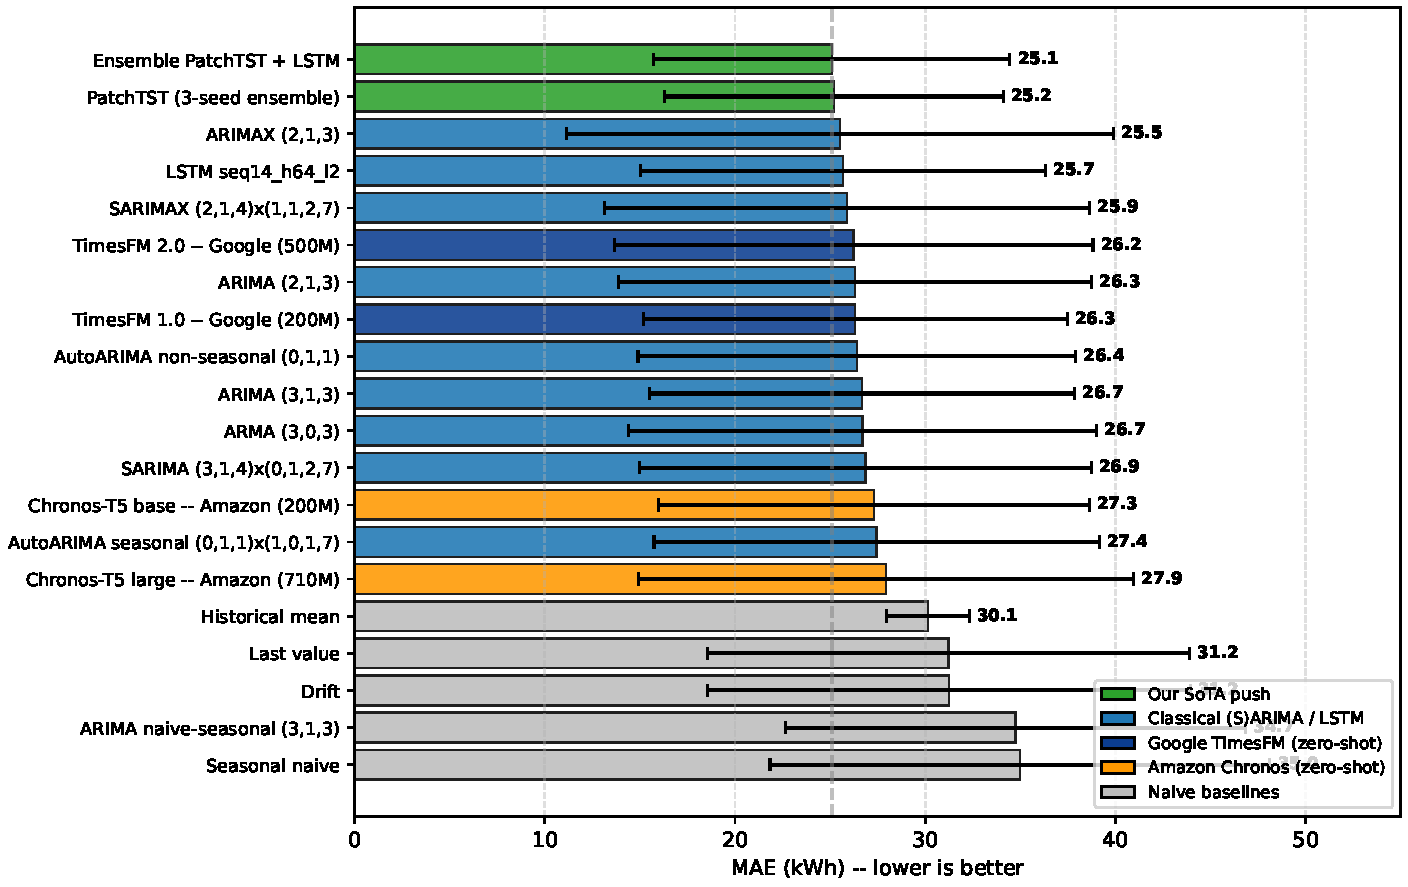
\includegraphics[width=0.95\textwidth]{fig_leaderboard}
\caption{Final leaderboard. Bars are MAE in kWh (lower is better);
error bars are one standard deviation across the four rolling-origin
windows. The Ensemble PatchTST + LSTM (top) is the best model
overall; the PatchTST seed-ensemble has the lowest std among
forecasting models.}
\label{fig:leaderboard}
\end{figure}

\subsection{Per-Window Analysis}

Figure~\ref{fig:per-window} breaks down the MAE by window for the top
six models. The takeaway here is window~3 (Nov 14--20, 2023), which
includes Thanksgiving: every model has its worst week here, with MAE
shooting up to 36--43~kWh. PatchTST is the one that loses the least
on that week (36.4~kWh vs.\ 38.8~kWh for the LSTM and $\sim$41~kWh
for ARIMAX), and that is the main reason it wins the leaderboard.
Outside window~3, the top models are essentially tied.

\begin{figure}[!htbp]
\centering
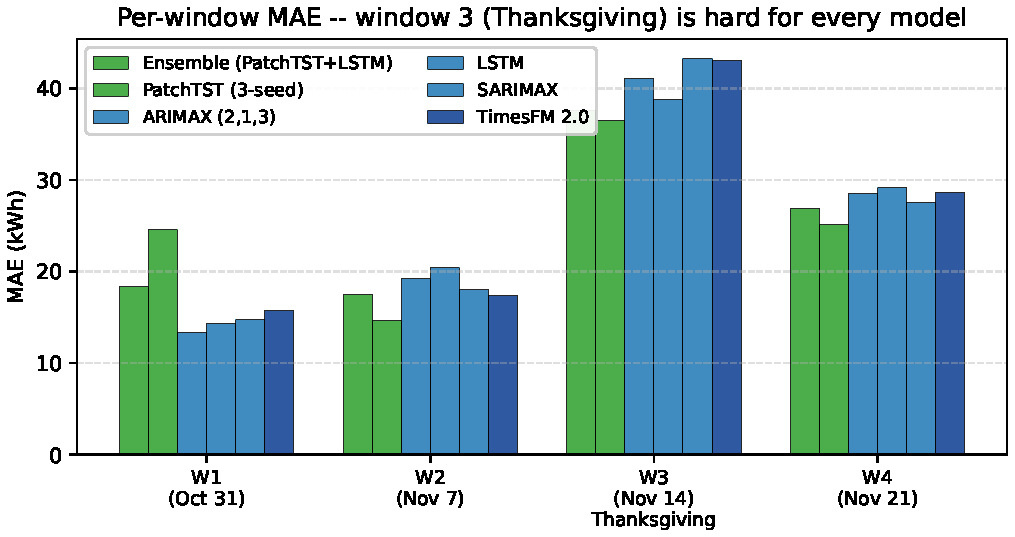
\includegraphics[width=0.95\textwidth]{fig_per_window}
\caption{Per-window MAE for the top six models. Window~3 (Thanksgiving
week) is hard for every model; the ranking on the other three windows
is much tighter. PatchTST loses less on the hard week, which is what
puts it (and its ensemble with LSTM) on top of the leaderboard.}
\label{fig:per-window}
\end{figure}

\subsection{Google vs.\ Amazon: Bigger Is Not Better}

The foundation-model rows of Table~\ref{tab:leaderboard} contain a
small surprise. Both Google TimesFM models clearly beat both Amazon
Chronos models (TimesFM 2.0: 26.23~kWh; Chronos-T5 large: 27.94~kWh,
the worst foundation model in our leaderboard). Inside each family
the size ordering is also informative: TimesFM 2.0 (500M) is only
marginally better than TimesFM 1.0 (200M), and Chronos-T5 large
(710M) is actually \emph{worse} than its smaller 200M sibling. Two
take-aways:
\begin{itemize}[leftmargin=*]
    \item \textbf{Foundation models do not win automatically.} The
    best foundation model (TimesFM 2.0) is at position 6 of our
    leaderboard, still beaten by ARIMAX, LSTM and SARIMAX in MAE.
    Zero-shot is a useful baseline but not a substitute for training
    on the target data.
    \item \textbf{More parameters means more prior, not more
    flexibility.} If the pre-training corpus is dominated by series
    that do not look like Boulder EV demand (random-walk-like
    financial series, for instance), a larger model amplifies the
    wrong prior. TimesFM transfers better because its pre-training
    mix includes more energy and load series; Chronos is trained on
    a different corpus and the larger checkpoint inherits more of
    that mismatch.
\end{itemize}

\subsection{What We Beat, and What We Did Not}

The honest claim, summarised:
\begin{itemize}[leftmargin=*]
    \item \textbf{Inside our protocol}, the Ensemble PatchTST + LSTM
    beats the strongest non-transformer model (ARIMAX) on both the
    mean MAE (25.09~vs.\ 25.52~kWh) and the standard deviation
    (9.36~vs.\ 14.38~kWh, ~35\% smaller). That is a real,
    apples-to-apples improvement.
    \item \textbf{Against the published literature}, no claim can be
    made in either direction. Koohfar~\cite{koohfar2023transformer},
    Wu~\cite{wu2025catformer} and
    Kyriakopoulos~\cite{kyriakopoulos2025comparative} all report
    metrics in normalised units (z-score or MinMax), on different
    station selections, and mostly on different horizons. Our 25~kWh
    and their 0.7--0.9 (normalised) are not in the same unit system.
\end{itemize}

\subsection{Stacking Did Not Work --- and Why}

For completeness we also tried two stacked meta-learners (Ridge and
NNLS, both leave-one-window-out, both trained on the six base learners
listed in Section~\ref{sec:models}). The results are in the middle
rows of Table~\ref{tab:leaderboard}: NNLS lands at 26.08~kWh MAE
(worse than the simple mean), and Ridge collapses to 32.29~kWh, which
is below several baselines. The reason is structural: 21 training
points per fold is not enough to fit reliable meta-weights. The Ridge
solution oscillates wildly between folds (we observed both very
negative and very large positive coefficients depending on which
window is held out), and NNLS concentrates almost all its weight on
the LSTM, throwing away the diversity the meta-learner was supposed
to exploit.

The dumbest combination wins: the unweighted mean of the two best
deep models, picked a priori. The lesson, which we re-state in
Section~\ref{sec:conclusions}, is that stacking needs a real
validation set --- not just a tiny held-out test set --- to learn
weights that generalise.


% -------------------------------------------------------
\section{Conclusions and Future Work}
\label{sec:conclusions}
\input{Sections/07_Conclusions}

% -------------------------------------------------------
\bibliographystyle{splncs04}
\bibliography{bibliography.bib}

\end{document}
